\thispagestyle{empty}
\chapter*{Acknowledgments}

This thesis is the final product, which in itself required a lot of effort, but the years during the doctoral process laid the foundation for everything. 
During this time, I have had the pleasure of meeting, learning from, researching with, and being supported by many great people, for which I would like to express my gratitude.

First of all, I would like to thank Bernhard Nebel, who not only gave me the opportunity to do my own research that interested me, but at the same time kept inspiring me with his expertise and dedication to topics like complexity theory.
The Foundations of Artificial Intelligence led by Bernhard was a great place to work with many wonderful people such as Florian Gei{\ss}er, Gregor Behnke, Grigorios Mouratidis, Johannes Aldinger, Petra Geiger, Robert Mattm{\"u}ller, Rolf-David Bergdoll, Stefan Staeglich, Thorsten Engesser, Tim Schulte and Uli Jakob, all of whom I would like to thank for great discussions and support. 

I would especially like to thank Robert Mattm{\"u}ller, who has supported and guided me since my first academic steps.
There are few people who can inspire young people with great commitment and enthusiasm for science. 
Among them, there are even fewer that allow young scientists to be seen as independent researchers by not putting themselves in the center of the action.
Robert is one of those few people without whom this work would not have been possible. Thank you very much.

I would like to thank all my colleagues with whom I have had the pleasure of writing, revising, and publishing a paper during my doctoral process: {\'A}lvaro Torralba, Andr{\'e} Biedenkapp, Bernhard Nebel, David Borukhson, Dominik Drexler, Florian Gei{\ss}er, Frank Hutter, Gregor Behnke, Jendrik Seipp, Marius Lindauer, Michael Katz, Robert Mattm{\"u}ller, Sumitra Corraya and Thomas Keller.
A special thanks to the planning community that has welcomed me since I first attended ICAPS 2018. 
In particular, to {\'A}lvaro Torralba for many interesting discussions, and to Michael Katz for the opportunity to work with him and visit the IBM T. J. Watson Research Center in New York. 
Both treated me like a colleague from the first meeting and shared their expertise with me.

Being a doctoral student is a roller coaster ride that is only possible with a well-balanced social life. 
I would like to take this opportunity to thank all my friends with whom I have shared many great experiences in my gymnastics career. 
Thanks to my study friends Andr{\'e} Biedenkapp, Lukas Gemein and Rick Gelhausen, all of whom will (hopefully) soon receive their PhDs. 
Special thanks to Andr{\'e} Biedenkapp, with whom I have shared many personally great times and scientific successes but also some setbacks.
The many overtime hours with you became a pleasure thanks to your positive attitude and enthusiasm for science.

I would like to thank my family. 
My parents Thomas and Olga, who have always supported me and taught me from an early age that hard work will pay off in the long run. 
They together with Iva, Mario and their slowly but steadily growing family were the support that many deserve but few receive. 
I am grateful that I can consider you not only family but also friends.

Last but not least, I would like to thank Lena (and Balu), who joined my journey a little later but are now indispensable. 
It is hard to describe how much I enjoyed the last time, although it should actually be very exhausting to write such a thesis. 
Lena, your incredibly loving, understanding and motivating nature towards me and my work has helped me to accomplish this thesis.

\vfill{}

\begin{center}
    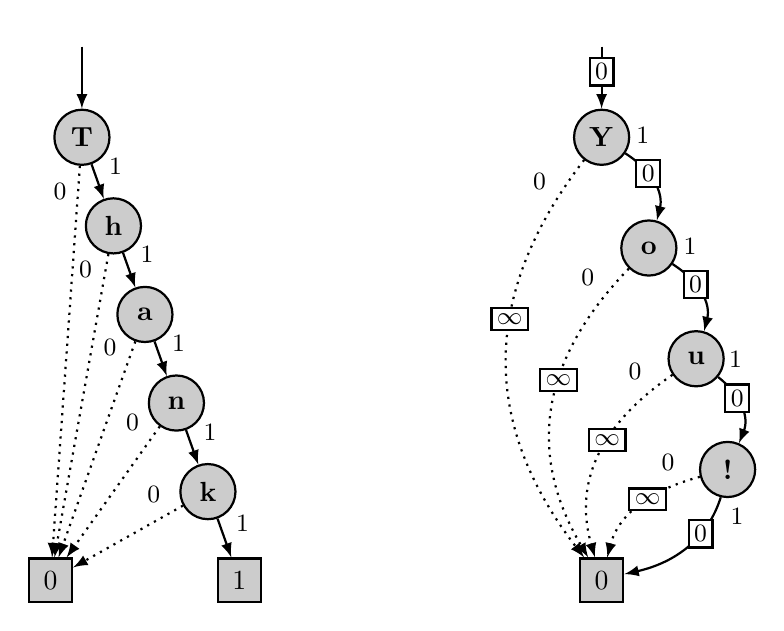
\begin{tikzpicture}[%
            costnode/.style={pos=0.6,rectangle,thick,solid,
                    inner sep=2pt,draw,fill=white,text=black,font=\small},%
            decisionnode/.style={circle,thick,minimum size=4mm,
                    inner sep=2pt,draw,fill=white!80!black,text=black,font=\normalsize},%
            xscale=2,yscale=1.5,>=latex]
        \begin{scope}{xshift=0cm}
            \node[] (before) at (0,4.6) {}; % incoming edge_value
            \node[decisionnode, minimum size=0.7cm] (t) at (0.0,3.75) {\textbf{T}};
            \node[decisionnode, minimum size=0.7cm] (h) at (0.2,3.0) {\textbf{h}};
            \node[decisionnode, minimum size=0.7cm] (a) at (0.4,2.25) {\textbf{a}};
            \node[decisionnode, minimum size=0.7cm] (n) at (0.6,1.5) {\textbf{n}};
            \node[decisionnode, minimum size=0.7cm] (k) at (0.8,0.75) {\textbf{k}};
            \node[draw,thick,fill=white!80!black,rectangle, minimum size=0.55cm]
            (after0) at (-0.2,0) {{$0$}};
            \node[draw,thick,fill=white!80!black,rectangle, minimum size=0.55cm]
            (after1) at (1.0,0) {{$1$}};
            \draw[->, thick] (before) to (t);
            % t =>
            \draw[->, thick] (t) to[bend right=0,label distance=0mm,edge
            label={\small{$1$}},pos=0.6] (h);
            \draw[->, thick, dotted] (t) to[bend left=0,label distance=0mm,edge
            label={\small{$0$}},swap,pos=0.1] (after0);
            % h =>
            \draw[->, thick] (h) to[bend right=0,label distance=0mm,edge
            label={\small{$1$}},pos=0.6] (a);
            \draw[->, thick, dotted] (h) to[bend left=0,label distance=0mm,edge
            label={\small{$0$}},swap,pos=0.1] (after0);
            % a =>
            \draw[->, thick] (a) to[bend right=0,label distance=0mm,edge
            label={\small{$1$}},pos=0.6] (n);
            \draw[->, thick, dotted] (a) to[bend left=0,label distance=0mm,edge
            label={\small{$0$}},swap,pos=0.1] (after0);
            % n =>
            \draw[->, thick] (n) to[bend right=0,label distance=0mm,edge
            label={\small{$1$}},pos=0.6] (k);
            \draw[->, thick, dotted] (n) to[bend left=0,label distance=0mm,edge
            label={\small{$0$}},swap,pos=0.1] (after0);
            % k =>
            \draw[->, thick] (k) to[bend right=0,label distance=0mm,edge
            label={\small{$1$}},pos=0.6] (after1);
            \draw[->, thick, dotted] (k) to[bend left=0,label distance=0mm,edge
            label={\small{$0$}},swap,pos=0.1] (after0);
        \end{scope}
        %\hfill
        \begin{scope}[xshift=3cm]
            \node[] (before) at (0.3,4.60) {}; % incoming edge_value
            \node[decisionnode, minimum size=0.7cm] (y) at (0.3,3.75) {\textbf{Y}};
            \node[decisionnode, minimum size=0.7cm] (o) at (0.6,2.8125) {\textbf{o}};
            \node[decisionnode, minimum size=0.7cm] (u) at (0.9,1.875) {\textbf{u}};
            \node[decisionnode, minimum size=0.7cm] (x) at (1.1,0.9375) {\textbf{!}};
            \node[draw,thick,fill=white!80!black,rectangle, minimum size=0.55cm]
            (after0) at (0.3,0) {{$0$}};
            \draw[->, thick] (before) to[bend right=0,label distance=0mm,edge
            label={},swap,pos=0.3] node[costnode,pos=0.4] {$0$} (y);
            % y =>
            \draw[->, thick, dotted] (y) to[bend right=30,label distance=0mm,edge
            label={\small{$0$}},swap,pos=0.1] node[costnode,pos=0.4] {$\infty$} (after0);
            \draw[->, thick] (y) to[bend left=30,label distance=0mm,edge
            label={\small{$1$}},pos=0.01] node[costnode,pos=0.35] {$0$} (o);
            % o =>
            \draw[->, thick, dotted] (o) to[bend right=30,label distance=0mm,edge
            label={\small{$0$}},swap,pos=0.1] node[costnode,pos=0.4] {$\infty$} (after0);
            \draw[->, thick] (o) to[bend left=30,label distance=0mm,edge
            label={\small{$1$}},pos=0.01] node[costnode,pos=0.35] {$0$} (u);
            % u =>
            \draw[->, thick, dotted] (u) to[bend right=30,label distance=0mm,edge
            label={\small{$0$}},swap,pos=0.1] node[costnode,pos=0.4] {$\infty$} (after0);
            \draw[->, thick] (u) to[bend left=30,label distance=0mm,edge
            label={\small{$1$}},pos=0.01] node[costnode,pos=0.35] {$0$} (x);
            % ! =>
            \draw[->, thick, dotted] (x) to[bend right=30,label distance=0mm,edge
            label={\small{$0$}},swap,pos=0.1] node[costnode,pos=0.4] {$\infty$} (after0);
            \draw[->, thick] (x) to[bend left=30,label distance=0mm,edge
            label={\small{$1$}},pos=0.01] node[costnode,pos=0.35] {$0$} (after0);
        \end{scope}
    \end{tikzpicture}
\end{center}

\vfill{}

